\documentclass[a4paper,12pt]{article}

\usepackage{amsmath,amsthm,amssymb,ae,aecompl,sgame,natbib,sgamevar,enumitem}
\usepackage[margin=2.5cm]{geometry}
\usepackage{tikz}
\usetikzlibrary{trees}

\title{Exercises Microeconomics}
\author{Christoph Schottm\"uller}
\date{}

\begin{document}
\maketitle
\section{Social choice}
\label{sec:social-choice}

\begin{enumerate}
\item Assume that there are at least 3 alternatives. Consider the following social welfare function: Alternatives are ranked according to points. The number of points of an alternative equals the number of agents that have this alternative as their top choice. Does this social welfare function satisfy (i) the weak Pareto principle, (ii) non-dictatorship, (iii) independence of irrelevant alternatives? Is it positive responsive?\footnote{For more than 2 alternatives, the definition of positive responsiveness has to be adapted: Say $x$ is weakly socially preferred, then $x$ should be strictly preferred if we improve $x$ in some agents preference order without changing the other agents' preference orders.}
  % violation of weak Pareto principle: let everyone have x>y>z, then y~z socially
  % violation of IIA: 2 people, 3 alternatives; preferences: x>y>z for both agents; compare to preferences z>x>y for both agents; individual ranking of x and y is same but socially we have x>y in first case and x~y in second;
  % violation positive responsiveness: agents 1: x>y>z; agent 2:y>z>x gives x~y>z socially; now change agent 2 to y>x>z then x is more preferred by him but social preference does not change
\item Assume that there are three alternatives $X=\{x,y,z\}$ and an odd number of agents with strict preferences. Consider the following procedure: First, a challenger is determined in a majority vote between $x$ and $y$. The loser of this vote is the least preferred alternative. The winner (i.e. the challenger) is put to a majority vote with the incumbent $z$. The winner of this second vote is the socially most preferred alternative and the loser the second most preferred. Does this social welfare function satisfy (i) the weak Pareto principle, (ii) non-dictatorship, (iii) independence of irrelevant alternatives?
  % violation of weak Pareto criterion: say all agents have preference x>y>z, then socially still z>y
  % violation of IIA: Condorcet example: P1 x>y>z, P2 y>z>x, P3 z>x>y; then socially z>x>y; now move x to the bottom of all people's preferences, i.e. P1 y>z>x, P2 y>z>x, P3 z>y>x and note that this leads to y>z socially though the ranking of z and y did not change individually
\item Let $X=\{x,y,z\}$ and $N=2$. Suppose whether $x$ or $y$ is better matters a lot for agent 1 and whether $y$ or $z$ is better matters a lot for agent 2. Therefore, the two agents have decided that the social ordering of alternatives between $x$ and $y$ should always be the ordering of agent 1 (i.e. $x\succeq_S y$ if and only if $x\succeq_1 y$) and similarly agent 2's ordering between $y$ and $z$ determines society's ordering of these two alternatives (i.e. $z\succeq_S y$ if and only if $z\succeq_2 y$). Show that given these two restrictions there is no social welfare function that satisfies the weak Pareto principle.\\(\emph{Hint: }Consider the rankings $x\succ_1 y$ and $y\succ_2 z$, determine the social preference relation and check whether there are complete preferences for the two agents such that this social welfare relation violates the weak Pareto criterion.)\footnote{This is a simplified version of exercise 6.13 in \cite{jehle2001advanced} in which you are asked to show a more general result. Armed with the solution of our exercise, you should be able to solve the more general problem if you put in a bit more work.}
  % take P1:z> x> y and P2: y>z>x; then the restrictions of the exercise imply the social preference x>y>z but x>z violates the Pareto criterion
  % for 6.13 in Jehle/Reny: let P1: z>x>y>w and P2: y>w>z>x. The Pareto criterion requires that socially z>x and y>w. As P1 is decisive for (x,y), we have socially  x>y and as P2 is decisive for (z,w)  we have w>z.But the first three relations imply by transitivity z>w. Contradiction! (Clearly, one can dd an arbitrary number of further alternatives and non-decisive agents. The latter are assigned the same preferences as either P1 or P2 in order not to interfere with the Pareto criterion. All other alternatives could, for example, be ranked below x,y,z,w by all agents.
\item Let $X=\{(0,0),(1,0),(0,1),(1,1)\}$, i.e. there are two related policy decisions which can be taken or not. Assume $N$ is odd and preferences are strict. Each individual finds the first decision more important; that is, if $(x,y)\succ_i (w,z)$ and $x\neq w$, then $(x,s)\succ_i (w,t)$ for any $s\in\{0,1\}$ and $t\in\{0,1\}$. Furthermore, each individual is consistent in the following sense:  $(0,y)\succ_i (0,z)$ if and only if $(1,y)\succ_i (1,z)$. Can you find a social welfare function that is non-dictatorial, satisfies IIA and the weak Pareto criterion? If yes, why does this not contradict Arrow's theorem?
  % the assumptions ensure that the outcome of pairwise majority voting are transitive, i.e. we do not run into the Condorcet problem. Say (a,b) beats (c,d) and (c,d) beats (e,f) in pairwise majority voting. We need to show that (a,b) beats (e,f). First, note that a\neq e: We cannot have a=c=e as then two of the alternatives would have to be the same. We also cannot have a=e\neq c because of the assumption that the first component is more important, i.e. if (a,b) beats (c,d) and a\neq c, then (a,f)=(e,f) beats (c,d). Second, we distinguish two cases: (i) a=c: then c\neq e and the assumption that the first dimension is more important together with the assumption that (c,d) beats (e,f) implies that (a,b)=(c,b) beats (e,f) in pairwise majority voting. (ii) a\neq c: then c=e but then the fact that (a,b) beats (c,d) and that the first dimension is more important implies that (a,b) beats (c,f)=(e,f).
\item Are the preferences in table \ref{tab:singlePeaked} single peaked?\\ If yes, add a fifth agent such that they no longer are single peaked. If no, find a three agent subgroup such that their preferences are single peaked. 
  \begin{table}[h]
    \centering
    \begin{tabular}{l|cccc}
        &most preferred& second most preferred& third most preferred& least preferred\\ \hline
      agent 1& w&z & x & y\\
      agent 2& z&y&w&x\\
      agent 3& x & w & z & y\\
      agent 4& z& w&x& y \\
    \end{tabular}
    \caption{Preferences}
    \label{tab:singlePeaked}
  \end{table}
  % order: y z w x (or opposite); add agent 5 y x z w
\item $N$ agents are living in a society. Agent $i$ has gross income $w_i$ (i.e. different agents have different incomes) and a cardinal utility function $u$ that depends only on his own net income, i.e. $u(w_i-t_i)$ where $t_i$ is the tax $i$ pays ($i$ can also get a subsidy which we will interpret as a negative tax). Assume that $u$ is strictly increasing and strictly concave and the same for all agents. Determine welfare maximizing taxes of all agents if the social welfare function is (i) Rawlsian welfare or (ii) utilitarian welfare. (Note that there is no outside source of funding, i.e. the sum of all taxes has to be zero.)\\
  Would the result change if $u$ was strictly increasing and linear?
  % (i) Rawls: ensure that w_i-t_i is the same for all agents as otherwise it would be optimal to redistribute money from someone with higher w_i-t_i to someone with lowest w_j-t_j which would increase W_Rawls as u is strictly increasing
  % (ii) $max_{t_1,\dots,t_N} \sum_i u(w_i-t_i)$ subject to $\sum_i t_i=0$. First order conditions show that $u_i'(w_i-t_i)$ is same for all agents and therefore everyone will have the same net income at the optimum, i.e. everyone has $w_i-t_i=(\sum_i w_i)/N$. This shows that utilitarian welfare as such is not against redistribution and the sometimes heard argument for Rawlsian welfare that it would better reflect preferences for redistribution is therefore flawed.
  % linear: no change for Rawls as strictly increasing u was all that was needed but now every allocation (that does not burn money) is optimal under utilitarian welfare
\item Consider a 2 person economy. We will use a diagram with utility of agent 1, $u_1$, on the horizontal and utility of agent 2 on the vertical axis. Assume that through the choice of appropriate options all $(u_1,u_2)$ pairs inside the unit circle (defined by $u_1^2+u_2^2\leq 1$) can be achieved.
  \begin{enumerate}
  \item Which achievable $(u_1,u_2)$ pairs are Pareto efficient?
    % the quarter of the unit circle in the positive quadrant
  \item Suppose you are maximizing the social welfare function $W=\alpha_1u_1+\alpha_2u_2$ with weights $\alpha_1,\alpha_2\in[0,1]$. Which $(u_1,u_2)$ pairs could (for some choice of weights) maximize $W$?
    % isowelfare curves have slope -\alpha_1/\alpha_2; hence, the welfare maximizing point is where the slope of the Pareto frontier equals -\alpha_1/\alpha_2. By using different $\alpha_1$ and $\alpha_2$ we can trace out the entire Pareto frontier. There is a more general result that this is always possible (under some mild regularity conditions). Hence, maximizing weighted utilitarian welfare can be used to determine the Pareto frontier (under some mild regularity conditions).
    \end{enumerate}
    
\end{enumerate}

\section{Markets and the first fundamental theorem of welfare economics}
\label{sec:mark-first-fund}

\begin{enumerate}[resume]
\item Consider a consumer and some given price vector $p$. The consumer demands more of good 1 than he initially has at this price vector, i.e. $x^i_1(p,m^i(p))>e^i_1$. Show that this consumer is worse off if the price of good 1 increases slightly (while all other prices remain the same). Would this still be the case if the price of good 1 increases a lot?
  % as $x_1$ is continuous, also after a small price increase the consumer has positive net demand. Let y be the optimal  consumption bundle at the new price vector. Then (p_1+epsilon)*(y_1-e^i_1)+ \sum_{j=2}^n p_j (y_j-e^i_j)=0 but this and y_1\geq e^i_1 implies that y was also feasible at price vector p. As $y$ was not chosen at p and the consumer maximization problem has a unique maximum, y is worse than whatever was chosen there -> consumer worse off.
  % for large price increases the consumer can become a net supplier of the good and be better off
\item Consider the following 2 agent, 2 good economy in which
  $$u^1(x_1,x_2)=x_1x_2 \qquad  e^1=(15,3)$$
  $$u^2(x_1,x_2)= log(x_1)+2 log(x_2) \qquad  e^2=(5,7).$$
  Derive the set of Pareto efficient allocations, determine the Walrasian equilibrium and the allocation in this equilibrium.\\
  (\emph{Hint:} Recall that (i) all of the endowment is consumed in an efficient allocation if utility is strictly increasing in each component and (ii) the marginal rate of substitution between the two goods has to be the same for the two agents in interior efficient allocations. Note that due to homogeneity of demand $p_1^*$ can be normalized, e.g., to 1. By Walras law, $z_2(p)=0$ if $z_1(p)=0$.)
  % efficiency: let $x_1$ and $x_2$ be consumption of agent 1, then agent 2 consumes 20-x_1 of good 1 and 10-x_2 in an efficient allocation. Equality of MRS gives x_2/x_1=(10-x_2)/(2*(20-x_1)) which can be rearranged as x_2=10x_1/(40-x_1). This curve goes through the two origins of the Edgeworth box and describes for x_1\in[0,20] the curve of efficient allocations.
  % The consumer problem of agent 1 has the first order conditions x_2-\lambda p_1=0 and x_1-\lambda p_2=0 which together with the budget constraint (x_1-15)p_1+(x_2-3)p_2=0 gives the solution x_1=(15p_1+3p_2)/(2p_1) and x_2=(15p_1+3p_2)/(2p_2).
  % The consumer problem for agent 2 has the focs 1/x_1-\lambda p_1=0 and 2/x_2-\lambda p_2=0 together with the budget constraint (x_1-5)p_1+(x_2-7)p_2=0 which gives the solution x_1=(5p_1+7p_2)/(3p_1) and x_2=(2*(5p_1+7p_2))/(3p_2).
  % aggregate demand is therefore for x_1: z_1(p)=(45p_1+9p_2+10p_1+14p_2-120p_1)/(6p_1) now normalize p_1^*=1 and solve for z_1(p^*)=0 which gives p_2^*=65/23; check that this also equates market 2: z_2(p)= (45p_1+9p_2+20p_1+28p_2-60p_2)/(6p_2)
  % equilibrium allocation: plug p^* into demand
\end{enumerate}

\section{Decision making under uncertainty}
\label{sec:decis-making-under}

\begin{enumerate}[resume]
  \item $L_1$ be throwing a fair dice: $C=\{1,2,3,4,5,6\}$, $p_i=1/6$ for $i=1,\dots,6$\\
$L_2$ be throwing an ``unfair dice'': $p_1=p_2=1/4$ and $p_3=p_4=p_5=p_6=1/8$\\
What is the probability that the outcome ``1'' occurs in the compound lottery $(L_1,L_2;1/2,1/2)$? Derive the reduced lottery of the compound lottery $(L_1,L_2;1/2,1/2)$.
% otucome 1: 1/2 * 1/6 + 1/2 * 1/4 = 5/24, outcome 3: 1/2 * 1/6 + 1/2 * 1/8 = 7/48; reduced lottery: (5/24, 5/24,7/48,7/48,7/48,7/48)
 \item  There are three prices:
  \begin{enumerate}
  \item 2.500.000 \$
  \item 500.000 \$
  \item 0 \$
  \end{enumerate}
An individual prefers the lottery $L_1=(0.1,0.8,0.1)$ to the lottery $L_1'=(0,1,0)$.\\
If the independence axiom is satisfied (as well as transitivity and monotonicity), which of the following lotteries does the individual prefer?\\
$L_2=(0.35,0.6,0.05)\qquad L_2'=(0.3,0.7,0)$
% L_2 = 0.5*L_1+0.5*(0.6,0.4,0) and L_2'=0.5*L_1'+0.5*(0.6,0.4,0). Hence, $L_2\succeq L_2'$ by independence axiom. 
  \item Let the preferences of a decision maker be represented by a von Neumann-Morgenstern utility function $U$ with Bernoulli utility function $u$. Show that the decision maker's preferences are also represented by the von Neumann-Morgenstern utility function $V$ with Bernoulli utility function $v(x)=a+b*u(x)$ for $b>0$ and $a\in \Re$.\footnote{You can show that this is not true for general $v(x)=\phi(u(x))$ where $\phi$ is a strictly increasing function. Take for example $u(x)=x$ and $\phi(z)=\sqrt{z}$. The decision maker with $u$ is then risk neutral while the one with $v$ is risk averse. E.g. take the two lotteries where $L$ pays 0 and 4 each with probability 0.5 and $L'$ pays 1.5 for sure. Then a decision maker with $u$ prefers $L$ while a decision maker with $v$ prefers $L'$. }
    % $L\succeq L'$ iff $\sum_i p_i u(x_i)\geq \sum_i p_i' u(x_i)$ which is equivalent to $a+b*\sum_i p_i u(x_i)\geq a+b* \sum_i p_i' u(x_i)$ for $a\in\Re$ and $b>0$. But the latter is equivalent to $\sum_i p_i (a+b*u(x_i))\geq \sum_i p_i' (a+b* u(x_i))$ which in turn is equivalent to $\sum_i p_i v(x_i)\geq \sum_i p_i' v(x_i)$.
\item The Bernoulli utility over money amounts be $u(x)=\sqrt{x}$. A decision maker has wealth 25 but loses 16 units of wealth with probability $1/2$.
  \begin{enumerate}
  \item What is the decision maker's expected wealth?
    % 0.5*25+0.5*(25-16)=17
  \item What is the expected utility of the decision maker?
    % 0.5*\sqrt{25}+0.5\sqrt{25-16}=4
  \item How much would the decision maker be willing to pay for an insurance that reimburses him his loss of 16 whenever it occurs?
    % under such an insurance the utility of the decision maker is $u(25-p)$ where $p$ is the insurance premium. The maximal $p$ DM is willing to accept is the one such that $u(25-p)=4$, i.e. his wtp is $9$.
  \item Find the willingness to pay for insurance in the graph of the lecture. 
    % distance between x_2 and the "certainty equivalent" which is defined by $u(CE)=E_L[u]$
  \item Find in the graph the amount by which the willingness to pay for insurance exceeds the expected loss. This amount is called the ``risk premium''. Why can this amount be interpreted as the scope for insurance? Show in the graph that the risk premium is low if the probability that a loss occurs is either very low or very high. What is the intuition?
    % RP = horizontal distance between orange dot and utility function; scope for insurance as this is the amount from which the administrative costs + profits of an insurer could stem; moving probability of loss move orange dot from one blue to the other; low and high prob of loss both correspond to relative certain environment while intermediate alpha is risky environment
  \item Answer the following in the graph: If the decision maker's Bernoulli utility is ``more concave'' between $x_1$  and $x_2$, i.e. a concave function passing through the two blue dots and lying above $u$ between $x_1$ and $x_2$, is the willingness to pay for insurance higher or lower?
    % higher as the certainty equivalent is lower; this is a general result: more concave Bernoulli utility means more risk aversion and therefore higher willingness to pay for insurance  
  \end{enumerate}
\end{enumerate}

\section{Bayesian Nash equilibrium}
\label{sec:bayes-nash-equil}

\begin{enumerate}[resume]
\item In a game show there are three closed doors. Behind one door there is a prize while there is no prize behind the other two doors. The participant will pick one door, say door 1. Then the host of the show will open another door behind which there is no prize, say door 2. The contestant can then decide whether he wants to stick to the door he initially chose (door 1) or switch to the other unopened door (door 3). He will then get what is behind the door he finally picked.
  \begin{enumerate}
  \item Assume that the prize is initially behind each door with probability 1/3. After the host opened the door, what are the probabilities that the prize is behind door 1 and door 3 respectively? Should the participant switch?
  \end{enumerate}
  % P[prize at d1|d2 open] = P[d2 open | prize at d1]*P[prize at d1]/(P[d2 open])  now:  P[d2 open | prize at d1]=1/2, P[prize at d1]=1/3, P[d2 open]=1/3*1/2+1/3*0+1/3*1=1/2 therefore P[prize at d1|d2 open]=1/3 while P[prize at d3|d2 open]=2/3 hence the participant should switch
  % intuitively compare from an ex ante point of view the two strategies "take a door and stay" and "take a door and switch". Clearly, the first strategy wins with probability 1/3 while the other strategy wins whenever the first strategy does not win, i.e. with prob 2/3.
\item Cournot competition with uncertain cost: There are two firms and each firm chooses a quantity $q_i$. Inverse market demand is $P(q_1,q_2)=1-q_1-q_2$. Firms have no fixed costs and marginal costs are $t_i$. The profit of each firm is therefore $(1-q_1-q_2-t_i)q_i$. Assume that costs $t_i$ are private information of firm $i$ and assume that $t_i$ equals $0.2$ with probability $1/2$ and $0.3$ with probability $1/2$ (and that the marginal costs of the two firms are independent). Determine a pure strategy BNE of this game.\\
  (\emph{Hint: }Check for a symmetric BNE in which the high types of the two players choose the same quantity, say $q^h$, and the low types of the two firms choose another quantity $q^l$.)
  % exp utility: 0.5*(1-q_i-q^h-t_i)q_i+0.5*(1-q_i-q^l-t_i)q_i leads to first order condition: 1-t_i-2q_i-q^ĥ/2-q^l/2=0. This has to be satisfied for t_i=0.2 and q_i=q^l as well as for t_i=0.3 and q_i=q^h. The two equations can be solve for q^l and q^h which gives q^l=11/40=0.275 and q^h=9/40=0.225
\item Take the public good example from the lecture with $N=3$. Find another BNE (this time an asymmetric one) in which player 1 never brings a speaker -- not even if he has a high type.
  % low types still never bring speaker; let \alpha be prob that P2 and P3 bring speaker if high type; then indiff condition $1/2 = 2\alpha/3$ and therefore $\alpha=3/4$, i.e. P2 and P3 bring a speaker with prob 3/4 if they are a high type and everything else never brings. Check that his strategy of not bringing is indeed optimal for the high type of P1 as given the others' strategies his expected utility of not bringing is 1-(1-2/3*3/4)^2=3/4>1/2.
\end{enumerate}

\section{Auctions}
\label{sec:auctions}

\begin{enumerate}[resume]
\item\label{ex:stratEq} Show that the following two situations are strategically equivalent, i.e. they lead to the same Bayesian game:
  \begin{enumerate}
  \item ``contest'': Each contestant $i$ (out of totally $I$ contestants) chooses how much effort $e_i$ to spend in the contest (e.g. how much time to spend on the task or how much money to spend in lobbying etc.). The contestant that spend the most effort will win the contest and receive a prize of value $v$. Effort is costly and costs contestant $i$ $\theta _ie_i$ where $\theta _i$ is private information of $i$ and drawn -- independently from other contestant's $\theta _j$ -- from a distribution $G$ with support on $[a,b]$ with $0<a<b$. The payoff of the winner is therefore $v-\theta _ie_i$ while the losers' payoff is $-\theta _ie_i$.
  \item ``all pay auction'': $I$ bidders bid (with weakly positive bids) for an object and the highest bidders gets the object. However, all bidders have to pay their bids (yes: also the losers pay!). The payoff of the winner is $v_i -b_i$ and the payoff of the losers is $-b_i$ where $b_i$ is the bid of player $i$, $v_i$ is private information of $i$ and drawn from a distribution $F$ with support on $[\underline{v},\bar{v}]$ with $0<\underline{v}<\bar{v}$.
  \end{enumerate}
  Find real-life examples that resemble the two situations.
  % set of players: {1,2}; strategy set: \Re_+; in contest let v_i=v/theta_i and write payoff as v_i-e_i (dividing by a positive constant, namely theta_i - does not change preferences); writing b_i instead of e_i gives the same payoff as in all pay auction and with \lowerbar=v/b and \bar v = v/a and G(v_i)=1-F(v/\theta_i) we get the same game as in all pay auction
  % competitive lobbying/bribing, patent races, sports competition, election campaigning
\item Derive the symmetric equilibrium of the first price auction with 2 bidders if the valuation of each bidder is drawn independently from a uniform distribution on $[0,2]$ (instead of $[0,1]$ as we did in the lecture). Do players shade their bids more or less? What is the intuition for this?\\
  (\emph{Hint:} Use the same steps as in the lecture but note that $v_j$ has a different distribution function. ``Guess'' a linear solution to the final differential equation.)
  % expected payoff is \beta^{-1}(b_i)/2 * (v_i-b_i) and the foc reads 1/(2\beta'(\beta^{-1}(b_i)))*(v_i-b_i)-\beta^{-1}(b_i)/2=0. If beta is sym. equilibrium maximum is achieved at b_i=\beta(v_i) ans therefore this can be written as $(v_i-\beta(v_i))/(\beta'(v_i))-v_i=0$. This differential equation is solved by $beta(v_i)=v_i/2$.
  % Intuition: it is like saying with prob 1/2 other's valuation is u[0,1] and with prob 1/2 other's valuation is u[1,2]. If v_i<1, then in the second case i looses anyway and therefore this has no impact on the effect of marginally changing b_i. The first case is, however, exactly the lecture!
\item\label{ex:allPay} Take the ``all pay auction'' in exercise \ref{ex:stratEq} and assume that $F$ is the uniform distribution on $[0,1]$ and $I=2$. Determine a symmetric equilibrium in strictly increasing strategies of this all pay auction. \\
  (\emph{Hint: }Proceed similarly as we did for the first price auction: write expected payoff from bidding $b_i$ assuming that the other bidder uses equilibrium strategy $\beta$, take the first order condition and use the fact that the first order condition has to hold at the equilibrium bid $\beta(v_i)$, solve the differential equation by ``guessing'')
  % Pr[b_i>\beta(v_j)] v_i-b_i = Pr[v_j<\beta^{-1}(b_i)] v_i-b_i = \beta^{-1}(b_i)v_i-b_i -> foc: v_i/(\beta'(\beta^{-1}(b_i)))-1=0 and therefore v_i=\beta'(v_i) which holds for beta(v_i)=v_i^2/2
%\item ``war of attrition'': $2$ people engage in an unpleasant task (like sitting in an unbearably hot room) and everyone has to choose a time $t_i$ when he will finish the task for everyone (e.g. by opening the window) if no one has done so before him. Finishing the task comes at cost $c>0$ while suffering up to time $t_i$ comes at cost $t_i\theta _i$ where  $\theta _i$ is private information of $i$ and drawn -- independently from the other player's $\theta _j$ -- from a uniform distribution on $[1,2]$. The payoff of person $i$ when being the one who ends the task at time $t_i$ is $-c-\theta _it_i$ while the other player has payoff $-\theta _jt_i$. Determine a symmetric equilibrium in strictly decreasing strategies.
 % (\emph{Hint: }Proceed similarly as we did for the first price auction: write expected payoff from bidding $b_i$ assuming that the other bidder uses equilibrium strategy $\beta$, take the first order condition and use the fact that the first order condition has to hold at the equilibrium bid $\beta(v_i)$)
 % Pr[t_i<\beta(\theta_j)] (c-t_i\theta_i)-  Pr[t_i>\beta(\theta_j)] \mathbb{E}[t_j|t_j<t_i]
\item Take the independent private value setting with 2 bidders and values uniformly distributed on $[0,1]$. Compare the revenue from an auction with the revenue from selling through the following two procedures:
  \begin{enumerate}
  \item posted price: the seller announces a posted price $p$ and buyers state whether they are willing to buy at price $p$. If at least one buyer is willing to buy, the good is sold at price $p$ to (one of) the willing buyer(s). At which prices is a buyer with valuation $v_i$ willing to buy? What are expected revenues as a function of $p$? Determine the revenue maximizing $p$.
    % buyers are willing to buy whenever v_i>p; Pr[sale]= 1- p^2;  revenues: p*(1-p^2) foc: 1-3p^2=0 and therefore p=\sqrt{\frac{1}{3}} and revenues are \sqrt{4/27}\approx 0.385
  \item sequential bargaining: the seller offers the good to buyer 1 at price $p_1$ and buyer 1 decides whether to buy or not. If he declines, the good is offered to buyer 2 at price $p_2$. Determine the revenue maximizing prices $p_1$ and $p_2$.
    % for p_2: max p_2(1-p_2), i.e. p_2=1/2 and expected revenue 1/4; for p_1: max (1-p_1)p_1+p_1*1/4 leading to foc: 1-2p_1+1/4=0 and therefore p_1=5/8; consequently revenue is 15/64+5/32=25/64\approx 0.391
  \item What tool is missing from our auction model? (i.e. how should a revenue maximizing seller sell his good?)
    % proper reserve price, i.e. we could incorporate the tool from (a) into our auction by setting a reserve price and have bidding above the reserve price to improve upon the revenue from (a)
  \end{enumerate}
\item (This exercise is a slightly simplified version of an exercise in \cite{klemperer2004auctions}.) In 1991 US Vice-President Quayle proposed that the loser in a lawsuit be required to transfer an amount equal to her own legal expenses to the winner. Quayle claimed this would reduce the amount spent on legal services (using the logic that one spends less if every dollar spent might cost another dollar). (Under current US rules each party pays its own costs.) We will model this by assuming each party $i=1, 2$ has a privately known value $v_i$, independently drawn from a uniform distribution on $[0,1]$, and the two parties simultaneously decide how much to spend on legal services. We assume that the party that spends the most money wins.
  \begin{enumerate}
  \item Use the revenue equivalence theorem to obtain the amount of money a player with value $v_i$ expects to spend in equilibrium under current US rules. What additional assumptions do you have to make for this approach to be valid?\\
    (Hint: using revenue equivalence to a sealed bid second price auction is probably simplest)
    % RET: same expected utility as in second price auction, there prob of winning is v_i and expected utility is v_i(v_i-v_i/2)=v_i^2/2
    % risk neutrality, symmetric equilibrium in strictly increasing strategies 
  \item Without any further calculations evaluate Quayle's claim that his proposal reduces legal expenditures. What additional assumptions do you have to make for your approach to be valid?
    % assume strictly increasing symmetric equilibrium and risk neutrality
    % note that lowest type has still zero utility as he spends zero in equilibrium; therefore revenue equivalence: same interim utility -> same expected expenses (but now including transfers); furthermore same incentives to bring cases to court as interim utility is unchanged.
    % 2 effects: higher incentive to win in order to get transfer and on the other hand bidding higher means that one has to transfer more when losing. under RET assumptions the two balance
  \item In some European countries, the loser pays a fraction of the winner's legal expenses. Assuming a fixed fraction $\alpha>0$, how will this rule affect legal expenses?
    % now the lowest types have a negative expected utility as they expect to pay a transfer but not to win; using the envelope theorem this actually means that in a symmetric equilibrium in strictly increasing strategies the costs of all types are higher (and interim utility is lower) than in the US because there is a higher incentive to win and no counter effect. However, this will affect which cases go to court...
  \end{enumerate}
%\item Take the all-pay-auction analyzed in exercise \ref{ex:allPay}. Derive again the equilibrium strategies of the players but this time use the revenue equivalence theorem and the results on either the FPA or the SPA on the slides  (instead of the players' first order condition).\\
%  (\emph{Hint:} What is the expected utility of a player in either auction format?)
%  by RET a bidder has the same expected utility as in the FPA. There he bids v_i/2 and wins with probability v_i, i.e. his expected utility is v_i(v_i-v_i/2)=v_i^2/2. expected utility in the all pay auction with strictly increasing bidding strategies is Prob[win]*v_i - b_i = v_i^2-b_i. Equating this with the expected utility in the FPA we get b_i=v_i^2/2.
\item Consider an auction in which the highest bidder gets the object and has to pay  0.5 times his own bid plus 0.5 times the bid of the second highest bidder (other bidders pay nothing). Assume independent, private values uniformly distributed on $[0,1]$ and $I=2$. Find the symmetric equilibrium of this auction. How does expected revenue compare to expected revenue of a second price auction?
  \\
  (\emph{Hint: }check linear bidding functions.)
  % by RET this auction is revenue and expected utility equivalent to a SPA and expected utility of a bidder with type v_i is v_i^2/2. The expected utility of a bidder in this auction is Pr[win](v_i-b_i/2-E[b_j/2|b_j<b_i])=v_i(v_i-b_i/2-E[b_j/2|v_i>v_j]). Equating this to v_i^2/2 yields 0=v_i/2-b_i/2-E[b_j/2|v_i>v_j] which is satisfied for b_i(v_i)=2v_i/3
\item Consider a take-over battle, i.e. two companies, say ``A'' and ``B'', want to take over a third company, say ``C''. Compare two scenarios: One in which the money paid to the previous owner of C in case of a successful take-over is partially tax deductible and one scenario where it is not. Who would benefit from the tax deduction?
  % If we assume that the take-over battle is in principle like an auction in which the higher bidder wins, and if we assume risk neutrality of the bidders, then RET applies and tells us that firms A and B are equally well off with and without the tax deduction. (Model the tax deduction as a partial reimbursement, e.g. you have to pay only half of your bid instead of the full bid in case of winning). Hence, bids will simply increase by the amount that firms can save in tax payments. However, this requires that both A and B have the same tax rate. Otherwise, a weaker bidder with a high tax rate might win against an - in principle - stronger bidder with a low tax rate, i.e. not the bidder with he highest valuation wins and the assumptions of RET would no longer be satisfied. In this case, bidders with high tax rates would benefit as their winning probabilities increase (see envelope theorem). Firm C definitely benefits from tax deduction for A and B as these lead to higher bids and more revenue for C (effectively financed by tax money).
\item Check that the equilibrium given in the slides for the first price auction with asymmetric bidders is indeed an equilibrium.\\
  (\emph{Hint: }Recall that the derivative of expected payoff in a first price auction with respect to one's own bid is $(v_i-b_i)\partial Pr[win]/\partial b_i-Pr[win]$ and verify that the first order condition holds for all types.)
  % for those types that do not win/loose for sure, \partial Pr[win]/\partial b_i=2 as the slope of both bidding functions is 1/2 and we have uniform distributions with density 1. The probability that bidder 1 wins is the probability that $b_1>v_2/2+1/6$ which using the uniform distribution of v_2 on [1,2] is 2b_1-1/3-1; hence the derivative of payoff with respect to b_1 is 2v_1-4b_1+4/3 which indeed is zero for b_1=v_1/2+1/3. For types where this bid is below the competitive range (i.e. the range of bids of bidder 2) we have a negative derivative for all competitive bids and therefore it is best to place a bid that never wins. Similar derivation for bidder 2.
\item Consider an independent private value auction with two bidders and uniformly distributed values on $[0,1]$. Assume that both bidders are budget constrained, i.e. they cannot pay more than 1/2. What are the implications for bidding? Will a first or a second price auction yield more revenue?  Why does the revenue equivalence theorem not hold?
  % no effect on first price auction as bidding b(v)=v/2\leq 1/2 is equilibrium there, i.e. constraint does not bind. However in SPA bidding one's valuation is not possible for bidders with v>1/2. As they cannot pay more than 1/2 all types above 1/2 can bid only 1/2. This is less than the unconstrained bids and therefore expected revenue is lower than in the unconstrained case while the FPA yields the same revenue as unconstrained. Hence, FPA yields more rvenue and RET does not hold as allocation is differently, i.e. in the SPA the highest valuation bidder does not necessarily win if both bidders have valuation above 1/2.
\item Consider the setting with asymmetric bidders on the slides. In this exercise we analyze reserve prices in this setting. Assume that the good is auctioned in a second price sealed bid auction.
  \begin{enumerate}
  \item Show that the revenue maximizing reserve price in this auction is 1.
    % In SPA equilibrium is to bid own valuation if this valuation is below reserve price and not bid otherwise. With a reserve price below 1 the strong bidder always wins and increasing the reserve price up to 1 increases revenue as it increases the price at which the strong bidder wins. If reserve prices are above 1, the weaker bidder cannot bid and some types of the stronger bidder are excluded as well. Clearly, the good is then always sold at the reserve price in case it is sold. Hence, expected revenues are in this case r*(2-r) which is maximized for r=1. 
  \item Suppose the auctioneer can set different reserve prices for the two bidders. Determine the revenue maximizing reserve prices $r_1$ and $r_2$.
    % Clearly $r_1\in[0,1]$ and $r_2\in[1,2]$. Hence, bidder 1 only wins if bidder 2's valuation is below the reserve price and his own valuation is above his reserve price. Whenever the good is sold, the trading price will be one of the reserve prices. Expected revenue is then $(2-r_1)r_1+(r_1-1)r_2(1-r_2)$ maximizing over $r_2$ yields the foc $1-2r_2=0$ or $r_2=1/2$. Maximizing over $r_1$ yields then the foc $2-2r_1+1/4=0$ or $r_1=9/8$
    % Note that in (a) effectively bidder1 was excluded. Now he is not excluded and as the auctioneer can make some revenue with bidder 1 it is optimal to exclude some types of the strong bidder in order to raise the price for the other types. Clearly, the reserve price for the weaker bidder is lower, i.e. the auctioneer wants to favor weaker bidders in order to maximize revenue (these observations are more general than our example in this exercise!).
  \end{enumerate}
  \item The British government auctioned licenses for electromagnetic spectrum that allowed the introduction of UMTS (``3G'', basically mobile internet) in 2000. Prior to the auction four companies operated in the mobile phone market but foreign mobile phone companies showed some interest in entering the market if they could provide UMTS services. It was initially unclear whether 4 or 5 licenses would be available. An expert council suggested an open ascending auction if 5 licenses were available (think of it, for simplicity, as an auctioneer raising the price until only 5 bidders are left and then selling the 5 licenses at this price) and the following Anglo-Dutch auction in case only 4 licenses were available. In the Anglo Dutch auction, there is a first phase with an open ascending auction until only 5 bidders are left. Then there is a second phase in which each of the 5 remaining bidders places a sealed bid (at least as high as the final price of the first phase) and the four highest bids win a license and have to pay the price they bid in the second phase. The goal of the government was an efficient allocation of licenses and -- as a secondary goal -- the generation of revenue.\\
    Why would the optimal form of auction depend on the number of licenses? What could have been the motivation of the expert council to suggest different designs for the two cases?\footnote{For more details and an extensive answer to this question, see  \citet[ch. 6]{klemperer2004auctions}.}
    % The 4 incumbents have an advantage as they can utilize their existing infrastructure. (Also there is a common value component suggesting that the advantage might matter a lot.) The ascending auction is similar to a SPA and a weaker bidder will never win there. With 4 licenses, it would therefore unlikely that one could motivate new entrants to bid. With 5 licenses motivating firms to enter the auction is not a problem as at least one entrant will get a license. The Anglo Dutch design tries to stimulate entry by having a FPA feature which gives weaker bidders a small chance of winning. Why not simply a sealed bid auction? The problem is that this can yield inefficient outcomes if bidders are asymmetric which they definitely were (entrants vs. incumbents etc.). There is a small risk of inefficiency in the Anglo-Dutch design (the fifth best bidder may get a license instead of the fourth best bidder) but this risk was judged to be small compared to the risk of having no serious entry (and very low revenue).
  \item In procurement auctions, bidders bid prices at which they are willing to procure a pre-specified service. The lowest bidder is contracted to provide the service at the price he bid. A reserve price is here a maximal bid, i.e. you are only allowed to bid lower prices. Consider the variable $\Delta$ which is defined in the following way: Take your bid minus the lowest bid of the other bidders divided by the reserve price. This gives a measure of how close you were to winning (if you did not win) or to losing (if you won) the auction. (We divide by the reserve price only to ``normalize'', i.e. to make projects of different sizes comparable.) Figure \ref{fig:distProcAucNat} gives the distribution of $\Delta$ for a large dataset of Japanese procurement auctions (taken from \cite{chassang2020robust}). 

    \begin{figure}[h]
      \centering
      \includegraphics[width=0.6\textwidth]{densProcAucNat.png}
      \caption{Distribution of $\Delta$}
      \label{fig:distProcAucNat}
    \end{figure}

    \begin{enumerate}
    \item What is unusual about this distribution?
      % around 0 the density drops substantially
    \item Suppose you prepare a bid and you expect a certain distribution of the strongest bids of your competitors. Call this distribution $G$ with a continuous density $g$. Can the bid that maximizes your expected profits, $b^*$, be such that $g(b^*)$ is very low?\\
      (Hint: write down your maximization problem and check the first order condition.)
      % max_b (1-G(b))(b-c) where c are your cost of procuring the service. foc: g(b^*)(b^*-c)=(1-G(b^*))  if g(b^*) is close to zero, the foc states that G(b^*)=1 which means you never win the auction, i.e. you bid the reserve price, which cannot be optimal unless you are the only bidder
      
    \item What do we conclude for the dataset depicted in figure \ref{fig:distProcAucNat}?
      % there is probably some collusion going on as such a distribution cannot be rationalized by competitive bidding
    \end{enumerate}
\end{enumerate}

\section{Adverse selection}
\label{sec:adverse-selection}

\begin{enumerate}[resume]
\item In the model of insurance demand assume that $i$ is uniformly distributed on $[1/4,3/4]$ and $\alpha=3/2$.
  \begin{enumerate}
  \item Determine $\mathbb{E}[i|i\geq\alpha p]$.
  \item Determine the equilibrium premium.
  \item Determine marginal costs, average costs and inverse demand and confirm the equilibrium by determining the intersection of average costs and inverse demand.
    \item Suppose buying insurance is subsidized by $s>0$. Determine the lowest subsidy for which full efficiency on the insurance market is reached.
    \end{enumerate}
  \item As a kid, I was told not to get into a stranger's car. In the age of Uber, Lift and so on, many of us voluntarily call strangers just to get into their cars. How does this relate to adverse selection and how did ride hailing platforms (try to) overcome this problem? Do you see similar problems and solutions outside the ride hailing sector?
    % those that want to rob/kidnap you have the highest benefits from getting you into their cars and should be the first ones to volunteer as drivers. Measures to counter this: record keeping and tracking, ratings, registration with biometrics of drivers and camera authentification of biometrics, (mic always on with automatic panic registration); registration and certification for traditional taxis
    % note also vice versa: those not wanting to pay may be the ones having most to gain from ride hailing (though this is also a common problem of traditional taxi drivers). here also rating systems might help
    % similar: AirBnB, ebay, etc.; online rating systems appear to have made these services viable
  \item A health insurance company considers adding birth preparation courses to its benefit package. The insurance company has 100 000 insured customers who gave birth to 1000 babys in the previous year. The added course will cost the insurance 200 € per participating couple and the company expects  50\% of the expecting couples to participate. By how much does the company have to increase its premium to cover the costs if the addition of the course should be profit neutral? Can you think of other situations (also outside the insurance sector) where similar effects play a role?\\
    (\emph{Hint:} This is not really a calculation exercise. You should think about and discuss the effects of the change.)
    % If the insurance pool stays the same and the number of babys per year remains stable, total costs would be 200*1000/2=100 000 and therefore raising the premium by 1 € would be profit neutral. However, you may expect the composition of the insurance pool to change as an effect of adding the course as a benefit, i.e. young women being or expecting to becoming pregnant find the insurance more attractive and others find it less attractive due to the increased premium. Hence, one should expect the share of mothers taking the course in the insured pool to increase as a response to the policy change. This means that the premium has to be increased by more than 1 € to keep profits constant. (There is a problem that this might trigger more non-mothers to leave the insurance etc., i.e. it is by no means clear that a profit neutral inclusion is possible.)
    % other decisions: suppose a political party (or other institution) changes an important policy stand: some opposing the change will leave and others welcoming the change will join the party, i.e. the fraction of party members welcoming the change will ex post be larger than ex ante (e.g. suppose the Catholic church allowed women to become priests etc. or the green party recategorised nuclear energy as "climate friendly" and supported it); think about a car manufacturer asking its customers whether they would buy an electric car -> after introducing it customer profile changes...
\end{enumerate}

\section{Weak perfect Bayesian equilibrium}
\label{sec:weak-perf-bayes}

\begin{enumerate}[resume]
\item Determine two pure strategy wPBE in the game depicted in figure \ref{fig:ex1}. Which of the two is a PBE?
  % Strategies: (L,A,l) belief: (1,0)
  % other  wPBE: (R,A,r) and belief (0,1)is  not a PBE as it does not induce a wPBE in the subgame starting at P2 (P3's belief has to be 1,0 there as only A is sequentially rational for P2)
  \begin{figure}[h]
\centering
% First, set the overall layout of the tree
% You might need to play with these sizes to ensure nothing overlaps.
\tikzstyle{level 1}=[level distance=1.5cm, sibling distance=3.5cm]
\tikzstyle{level 2}=[level distance=1.5cm, sibling distance=3.5cm]
\tikzstyle{level 3}=[level distance=1.5cm, sibling distance=2cm]
\tikzstyle{level 4}=[level distance=1.5cm, sibling distance=1.5cm]
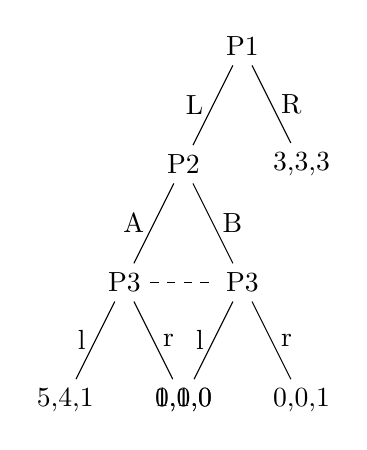
\begin{tikzpicture}
%Start with the parent node, and slowly build out the tree
% with each "child" representing a new level of the diagram
% each "node" represents a labelled (or unlabeled if you 
% want) node in the diagram.
\node{P1}
    child{
             node{P2}
             child{
               node(a){P3}
                  child{
               node{5,4,1}
               edge from parent
               node[left]{l}
               }
             child{
               node{1,1,0}
               edge from parent
               node[right]{r}
               }
               edge from parent
               node[left]{A}
               }
             child{
               node(b){P3}
                  child{
               node{0,0,0}
               edge from parent
               node[left]{l}
               }
             child{
               node{0,0,1}
               edge from parent
               node[right]{r}
               }
               edge from parent
               node[right]{B}
               }
           edge from parent
           node[left]{L}
           }
    child{
         node{3,3,3}
         edge from parent
         node[right]{R}
         };
\draw [dashed](a)--(b);
\end{tikzpicture}
\caption{Exercise 1}
\label{fig:ex1}
\end{figure}

  \item This exercise deals with the game of figure \ref{fig:selten_ex} which Reinhard Selten -- the only Nobel laureate in economics from Germany -- introduced to illustrate that subgame perfection was not enough to rule out non-credible threats.
    \begin{enumerate}
    \item Transform this game into its ``normal form'' (i.e. a game table) and find a pure strategy Nash equilibrium. Show that this equilibrium is subgame perfect. Show that this NE is, however, not sequentially rational. 
    \item Find a wPBE using mixed strategies.\\ (\emph{Hints:} What action is sequentially rational for player 2? For which belief is player 3 willing to mix? Under which circumstances is player 1 willing to mix?)
    \end{enumerate}
    \begin{figure}[h]
\centering
% First, set the overall layout of the tree
% You might need to play with these sizes to ensure nothing overlaps.
\tikzstyle{level 1}=[level distance=0.75cm, sibling distance=6cm]
\tikzstyle{level 2}=[level distance=1.5cm, sibling distance=2.5cm]
\tikzstyle{level 3}=[level distance=1.5cm, sibling distance=2cm]
\tikzstyle{level 4}=[level distance=1.5cm, sibling distance=1.5cm]
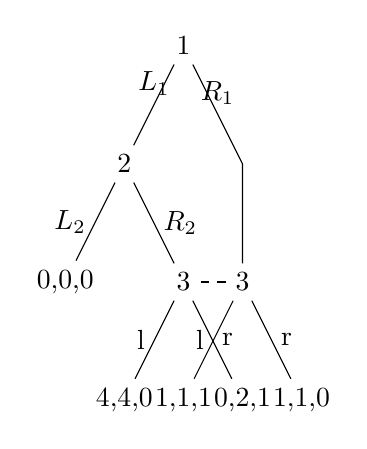
\begin{tikzpicture}
%Start with the parent node, and slowly build out the tree
% with each "child" representing a new level of the diagram
% each "node" represents a labelled (or unlabeled if you 
% want) node in the diagram.
\node{1}
    child{
             node{2}
             child{
               node{0,0,0}
             edge from parent
             node[left]{$L_2$}}
             child{
               node(b){3}
                  child{
               node{4,4,0}
               edge from parent
               node[left]{l}
               }
             child{
               node{0,2,1}
               edge from parent
               node[right]{r}
               }
                edge from parent
                node[right]{$R_2$}
               }
           edge from parent
           node[left,above]{$L_1$}
           }
    child{
           child{
               node(c){3}
                  child{
               node{1,1,1}
               edge from parent
               node[left]{l}
               }
             child{
               node{1,1,0}
               edge from parent
               node[right]{r}
               }
               }
         edge from parent
         node[right,above]{$R_1$}
         };
\draw [dashed](c)--(b);
\end{tikzpicture}
\caption{Selten's horse}
\label{fig:selten_ex}
\end{figure}

\item Take the model of ``Coasian dynamics'' on the slides but assume that $\delta=1/2$.
  \begin{enumerate}
  \item Show that the wPBE from the lecture is no longer a wPBE if $\delta=1/2$.
    % seller could deviate p_1=p_2=8 and sell in period 2 only to high value types which yields an exp. payoff of 0.5*(0.5*8)=2>1 and is therefore profitable. Hence seq rat is violated.  
  \item Verify that the other strategy profile on the slides (where $p_1=8$ and $p_2=1$) is also not a wPBE.
    % type 9 buyer could profitably deviate by choosing not to buy in period 1 but only int period 2 which gives an expected payoff of 0.5*(9-1)=4>1
  \item Determine a wPBE in mixed strategies.\\
    (\emph{Hint:} For which belief would the seller be willing to mix over prices in period 2? How would the buyer of type 9 have to mix in period 1 to justify this belief? Under which circumstances would a type 9 buyer be willing to mix in period 1?)
    % seller is indifferent for \mu_2=1/8; if low value buyer does not buy in period 1 and the high value buyer buys with probability 6/7 then in \mu_2=0.5*1/7/(0.5*1/7+0.5*1)=1/8
    % To make type 9 indifferent in period 1: p_1=8 while in period 2 seller chooses p_1=8 with probability q such that 9-8=0.5*(q*(9-8)+(1-q)*(9-1)), i.e. q=6/7.
    % wPBE:
       %seller: p_1=8 while p_2=8 with prob 6/7; \mu_2=1/8
       %buyer: type 2 buys whenever price is 1, type 9 buys whenever price is 1 and with prob 6/7 in period 1 if p_1=8 and at any price in period 2
  % note that this is seq. rational for seller, i.e. his expected profits in eq. are 8*0.5*6/7+0.5*(1*(0.5+0.5*1/7))=26/7 while deviating in period 1 to p_1=1 would yield 1  
  \end{enumerate}
\end{enumerate}

\section{Signaling}
\label{sec:signaling}

\begin{enumerate}[resume]
\item In the job market signaling model assume $c(e,\theta )=(1-\theta) e^2/6$ together with $\lambda=1/2$, $\theta _h=3/4$ and $\theta _l=1/4$.
  \begin{enumerate}
  \item Determine the least cost separating equilibrium.
    % rearranging 1/4=3/4-0.75*e^2/6 gives \tilde e=2 while e_l=0, w(0)=1/4, w(\tilde e)=3/4. Example mu: \mu(e)=0 if e<\tilde e and \mu(e)=1 else
  \item Determine all separating equilibria.
    % rearranging 1/4=3/4-0.25 e^2/6 gives \bar e=\sqrt{12}. Any e_h\in[\tilde e,\bar e] together with e_l=0 and \mu(e)=0 for e< e_h and \mu(e)=1 else is sep eq.
  \item Determine all pooling equilibria.
    % E[\theta]=1/2; rearranging 1/4=1/2-0.75 e^2/6 gives e'=\sqrt{2}, hence any e_p\in[0,e'] with \mu(e)=0 for e< e_p and \mu(e)=\lambda else is pooling eq
  \item Now concentrate on the least cost separating equilibrium. Assume a revenue neutral tax scheme with a tax on high incomes of $1/20$ is introduced. What is the subsidy on for low incomes to make the scheme revenue neutral? What is the equilibrium education level with the tax? Are high types better or worse off with the tax?
    % s=t*0.5/0.5=t=0.05; rearranging  1/4+0.05=3/4-0.05-0.75 e^2/6 gives e_h^t=\sqrt{3.2}; payoff of high type without tax: 3/4-0.25*4/6=7/12 while with the tax their payoff is 3/4-0.05-0.25*3.2/6=0.7-2/15=17/30<7/12 and therefore high types are better off without the tax
  \item Again focusing on least cost separating equilibria, for which values of $\lambda$ are high types better off without a tax of $t=0.05$?
    % s=0.05*\lambda/(1-\lambda). Define r=\lambda/(1-\lambda), then e_h^t is determined by 1/4+0.05r =3/4-0.05-0.75 e^2/6 or e_h^t=\sqrt{3.6-0.4r} and consequently the payoff of a high type is 3/4-0.05-0.25*(3.6-0.4r)/6=0.55+r/60; equating this with the payoff without tax, i.e. 7/12, yields the critical r=2 or equivalently the critical lambda=2/3. Hence, theta_h is better off with the tax if \lambda>2/3 and better off without the tax otherwise
  \end{enumerate}
\item Suppose you want to signal that you are physically strong. What could be suitable signals?
  % not suitable: gym membership card as anyone can get this or having a triathlon starting number on your arm; suitable: carrying around dumbbells 
\end{enumerate}

\newpage
\bibliographystyle{chicago}
\bibliography{/home/christoph/stuff/bibliography/references.bib}


\end{document}